\section{实验三 使用快速傅里叶变换进行频谱分析}

\subsection{一、实验目的}
1. 加深对FFT、频谱混叠、频谱泄漏现象的理解；
2. 掌握基于FFT对典型离散信号做频谱分析的MATLAB实现方法；
3. 学会利用FFT快速计算线性卷积；
4. 掌握不同采样率、序列补零对FFT频谱结果的影响；
5. 熟悉FFT工程仿真编程与波形绘图规范；
6. 掌握音符合成乐曲、ADSR包络降噪、音频生成与频谱分析方法。

\subsection{二、实验原理}
1. 离散傅里叶变换DFT实现频域分析，FFT是DFT快速优化算法，MATLAB \texttt{fft()} 可直接完成运算；
2. 时域卷积等价于频域相乘，可通过「FFT→频域相乘→IFFT」实现线性卷积；
3. 时域采样不满足奈奎斯特准则会发生频谱混叠；信号截断有限长会产生频谱泄漏；序列末尾补零仅细化频谱刻度，不提升频率分辨率。
4. 分段音符直接拼接存在相位跳变，引入ADSR（起音-衰减-保持-释放）包络调制幅值可消除间断毛刺；叠加高次谐波可模拟真实乐器音色。

\subsection{三、实验内容}
1. 构造三角脉冲、矩形脉冲离散序列，FFT求解双边幅度谱、相位谱并绘图分析；
2. 利用FFT频域相乘方法实现两组序列线性卷积，与时域\texttt{conv()}、圆周卷积\texttt{cconv()}结果对照验证；
3. 多组采样率对双频正弦混合信号采样，观测频谱混叠现象；对比64点补零延拓、直接128点采样两种FFT频谱差异；
4. 音乐合成趣味实验：按曲谱音符基频生成正弦音频；对比无包络、ADSR包络、叠加谐波+ADSR包络三种波形；导出wav音频，对比时域波形与频谱差异。

\subsection{四、实验结果}
\begin{figure}[H]
\centering
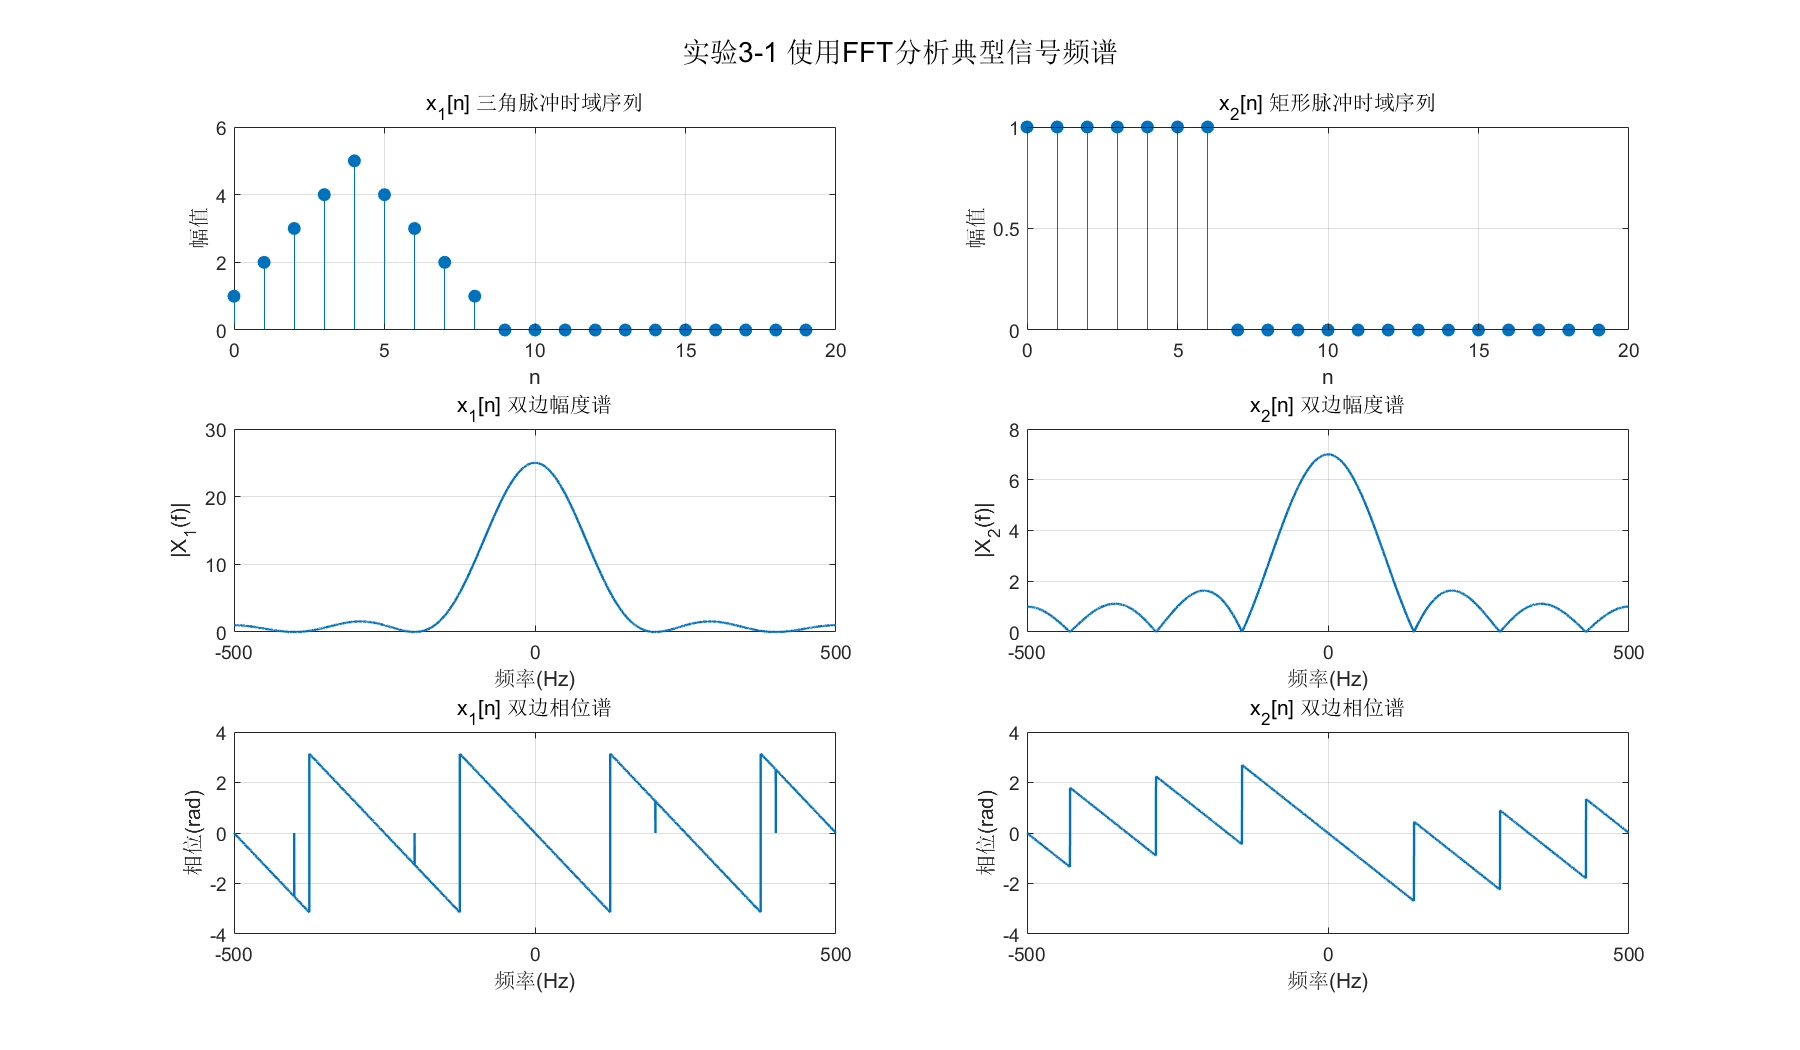
\includegraphics[width=0.9\textwidth]{3.1.png}
\caption{三角、矩形脉冲时域、双边幅度谱、双边相位谱对比}
\end{figure}

\begin{figure}[H]
\centering
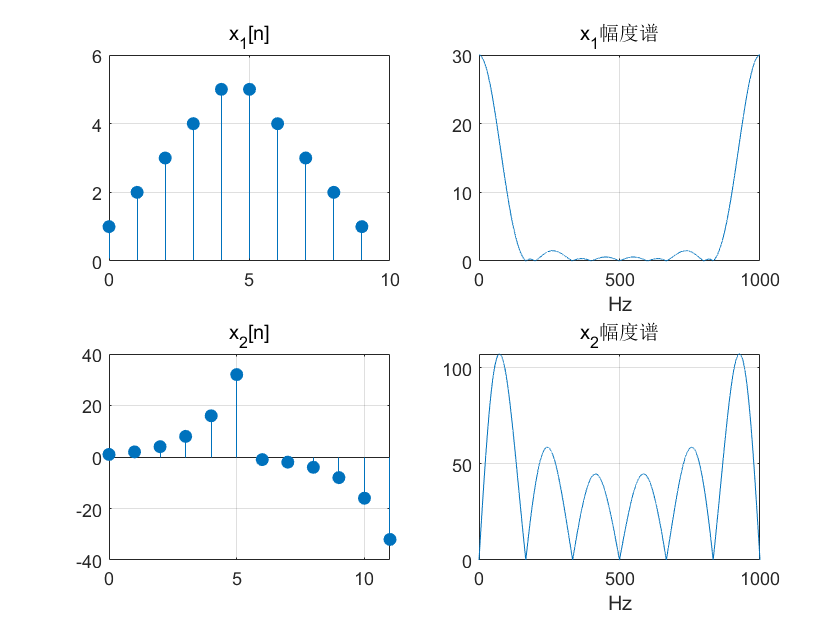
\includegraphics[width=0.9\textwidth]{3.2.1.png}
\caption{第一组原始序列时域及对应幅度谱}
\end{figure}

\begin{figure}[H]
\centering
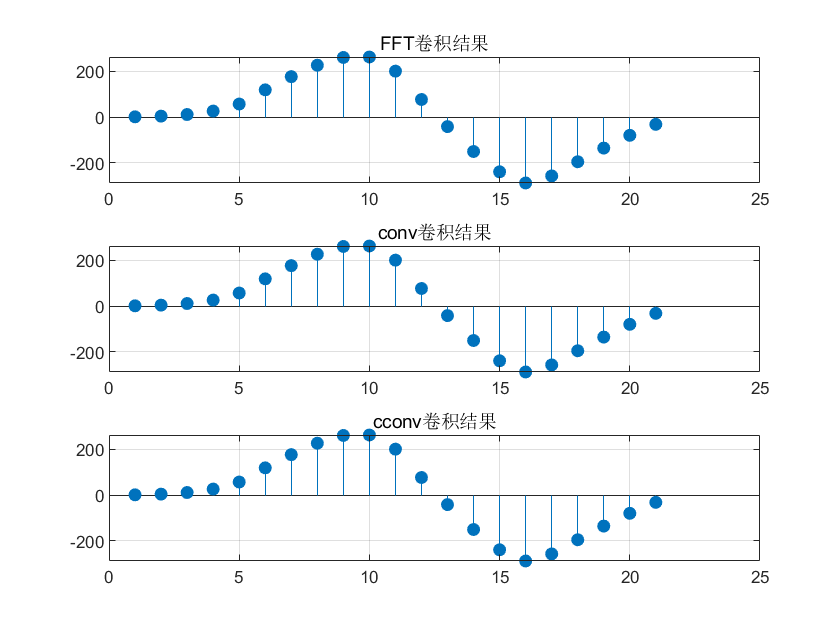
\includegraphics[width=0.9\textwidth]{3.2.2.png}
\caption{第一组FFT/conv/cconv卷积时域结果对比}
\end{figure}

\begin{figure}[H]
\centering
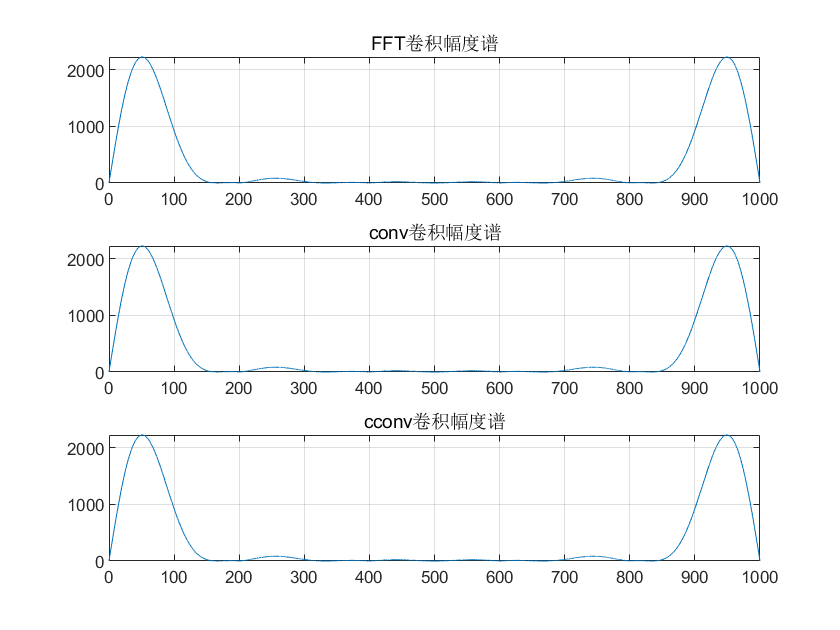
\includegraphics[width=0.9\textwidth]{3.2.3.png}
\caption{第一组三种卷积结果幅度谱对比}
\end{figure}

\begin{figure}[H]
\centering
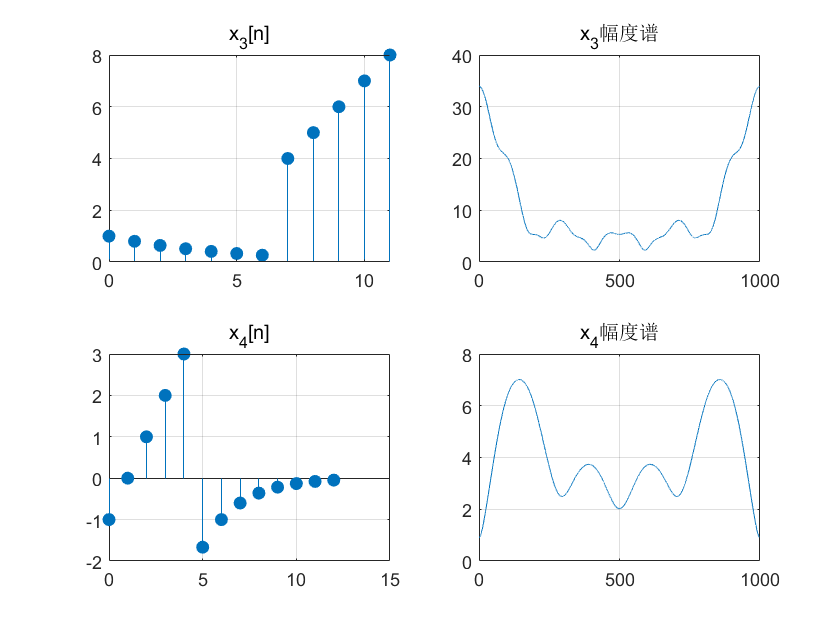
\includegraphics[width=0.9\textwidth]{3.2.4.png}
\caption{第二组原始序列时域及对应幅度谱}
\end{figure}

\begin{figure}[H]
\centering
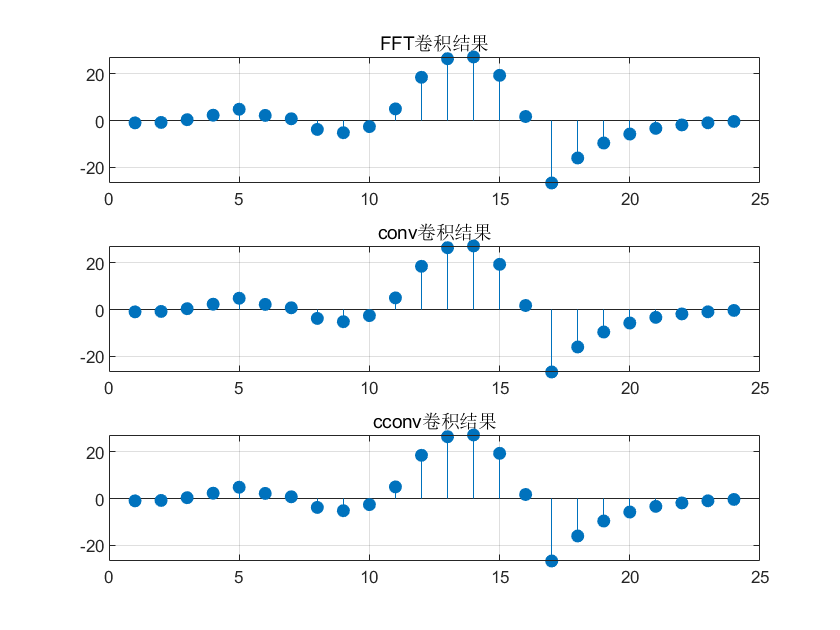
\includegraphics[width=0.9\textwidth]{3.2.5.png}
\caption{第二组FFT/conv/cconv卷积时域结果对比}
\end{figure}

\begin{figure}[H]
\centering
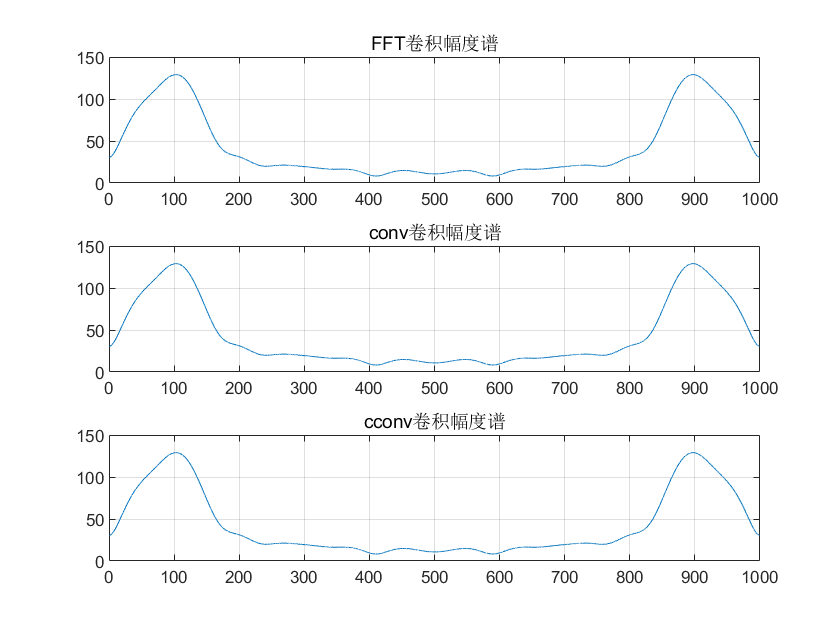
\includegraphics[width=0.9\textwidth]{3.2.6.png}
\caption{第二组三种卷积结果幅度谱对比}
\end{figure}

\begin{figure}[H]
\centering
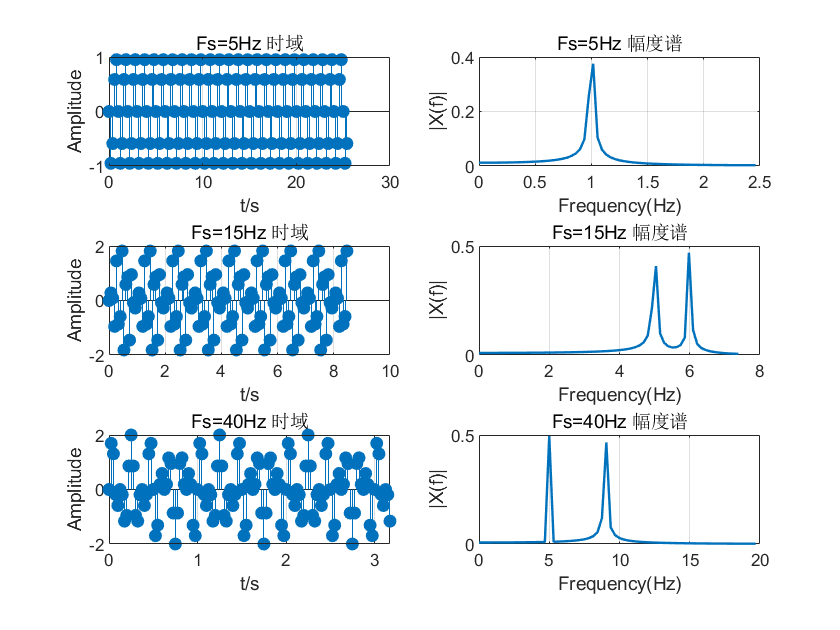
\includegraphics[width=0.9\textwidth]{3.3.1.png}
\caption{3种采样率下信号时域波形与幅度谱（频谱混叠观测）}
\end{figure}

\begin{figure}[H]
\centering
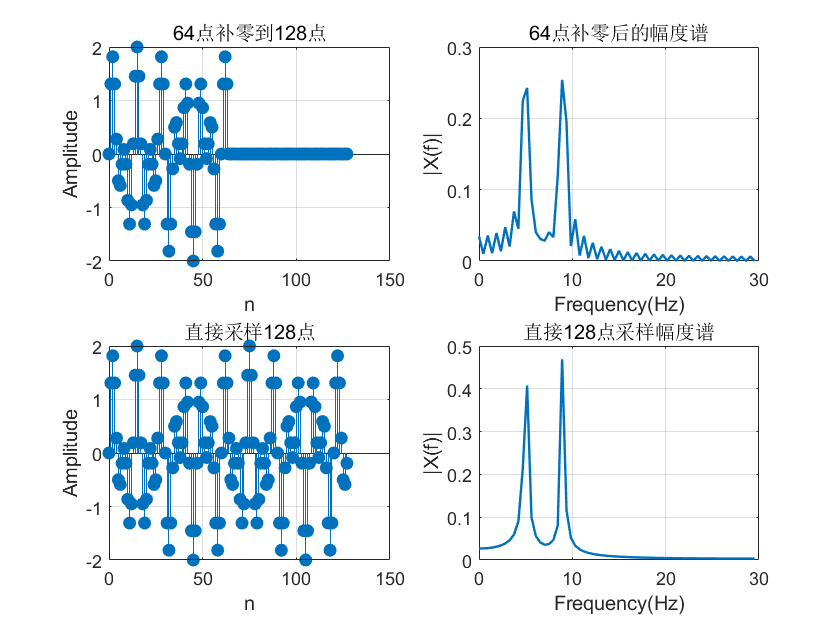
\includegraphics[width=0.9\textwidth]{3.3.2.png}
\caption{64点补零延拓与直接128点采样时域、频谱对比}
\end{figure}

\begin{figure}[H]
\centering
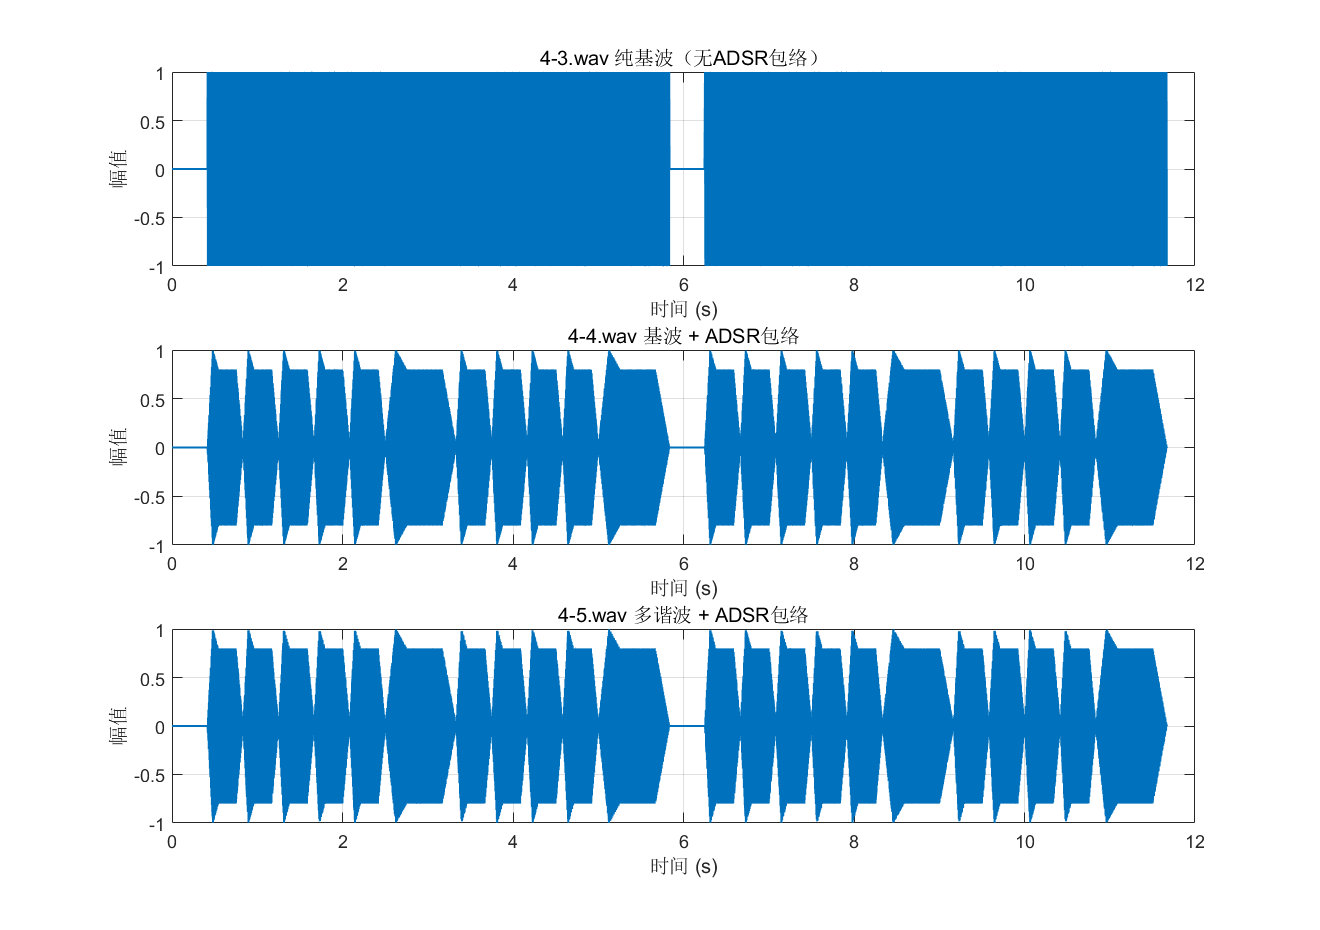
\includegraphics[width=0.9\textwidth]{3.4.1.png}
\caption{三段合成音乐时域波形对比}
\end{figure}

\begin{figure}[H]
\centering
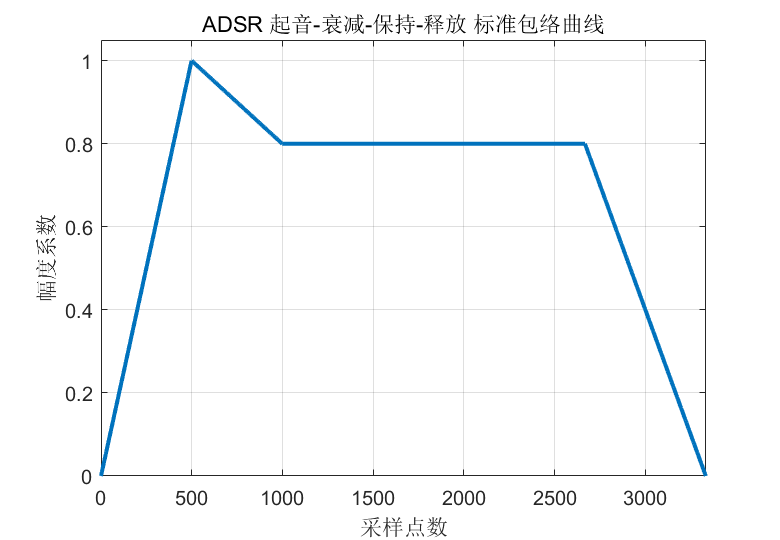
\includegraphics[width=0.7\textwidth]{3.4.2.png}
\caption{标准ADSR四段包络曲线}
\end{figure}

\begin{figure}[H]
\centering
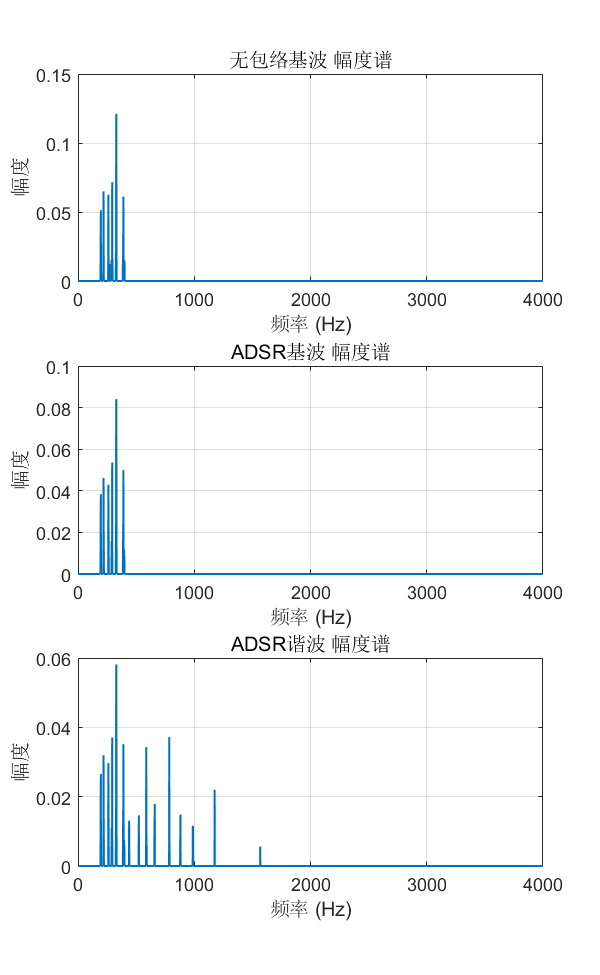
\includegraphics[width=0.9\textwidth]{3.4.3.png}
\caption{三组音频幅度谱对比}
\end{figure}

\begin{figure}[H]
\centering
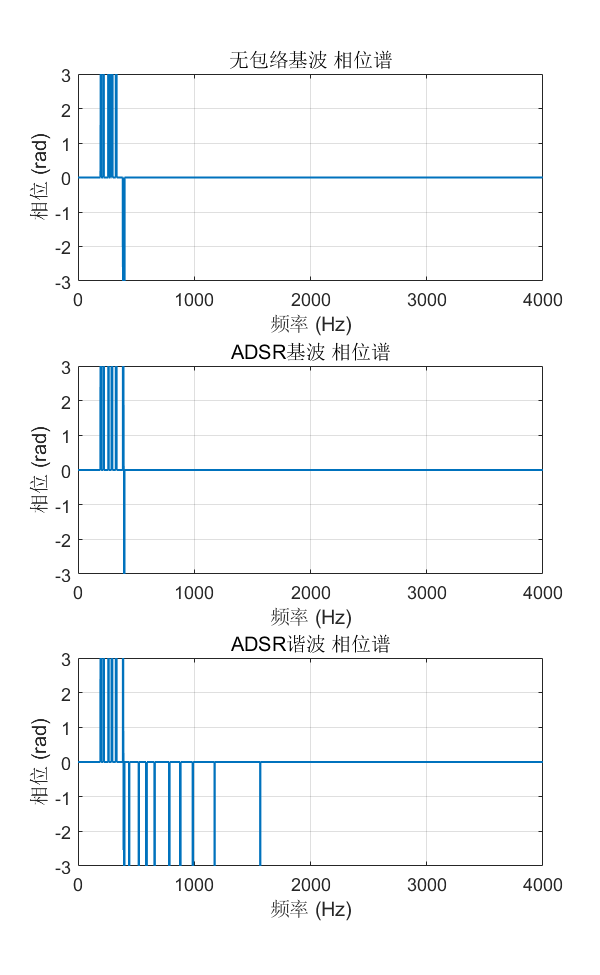
\includegraphics[width=0.9\textwidth]{3.4.4.png}
\caption{三组音频相位谱对比}
\end{figure}

\subsection{五、实验结论}
1. 矩形脉冲、三角脉冲频谱形态存在明显区别，有限长截断都会产生频谱泄漏；fftshift做双边谱后频谱关于0Hz对称，零频分量位于图像中心；
2. FFT频域相乘可以等效实现线性卷积，只要FFT长度满足$L\ge L_1+L_2-1$，IFFT取实部后结果和\texttt{conv()}完全一致，运算效率远高于时域直接卷积；圆周卷积长度选取合适时也等价于线性卷积；卷积后频谱等于两个输入信号频谱逐点相乘；
3. 采样频率低于奈奎斯特频率时高频分量折叠进低频区间，出现频谱混叠；对短序列末尾补零只能插值平滑频谱曲线、细化横坐标刻度，不能提升真实频率分辨率；增加有效采样点数才能提高频率分辨率；
4. 音符直接拼接时域存在幅值跳变毛刺，播放出现“啪”噪声；加入ADSR渐变包络后幅值平滑过渡，间断噪声消除；叠加多次谐波后频谱多出谐波分量，音色更贴近真实乐器；导出的三段wav音频可正常播放，时域与频谱特征区分明显。

\subsection{六、MATLAB完整实验代码}
\subsubsection{实验3-1 典型脉冲FFT频谱分析 exp3\_1.m}
\begin{lstlisting}
%% exp3_1.m
% 实验3-1 FFT典型脉冲频谱分析（双边谱）

clear;
clc;
close all;

%% =========================
% 参数设置
%% =========================

fs = 1000;      % 采样频率
N  = 10000;     % FFT点数

%% =========================
% 构造三角脉冲 x1[n]
%% =========================

x1 = zeros(1,N);

for n = 0:N-1

    if n>=0 && n<=4
        x1(n+1)=n+1;

    elseif n>=5 && n<=8
        x1(n+1)=9-n;

    else
        x1(n+1)=0;
    end

end

%% =========================
% 构造矩形脉冲 x2[n]
%% =========================

x2 = zeros(1,N);

for n = 0:N-1

    if n>=0 && n<=6
        x2(n+1)=1;

    else
        x2(n+1)=0;
    end

end

%% =========================
% FFT
%% =========================

X1 = fft(x1,N);
X2 = fft(x2,N);

%% =========================
% 双边谱处理
%% =========================

X1_shift = fftshift(X1);
X2_shift = fftshift(X2);

%% 幅度谱

A1 = abs(X1_shift);
A2 = abs(X2_shift);

%% 相位谱

P1 = angle(X1_shift);
P2 = angle(X2_shift);

%% 去除极小值处相位抖动

P1(A1<1e-6)=0;
P2(A2<1e-6)=0;

%% =========================
% 双边频率轴
%% =========================

f = (-N/2:N/2-1)*(fs/N);

%% =========================
% 绘图
%% =========================

figure('Name','实验3-1 FFT典型脉冲频谱分析',...
       'Color','w',...
       'Position',[100 100 1200 700]);

%% ---------- 第一列：三角脉冲 ----------

subplot(3,2,1)

stem(0:19,x1(1:20),'filled');
grid on;

xlabel('n');
ylabel('幅值');

title('x_1[n] 三角脉冲时域序列');

subplot(3,2,3)

plot(f,A1,'LineWidth',1.2);

grid on;

xlabel('频率(Hz)');
ylabel('|X_1(f)|');

title('x_1[n] 双边幅度谱');

subplot(3,2,5)

plot(f,P1,'LineWidth',1.2);

grid on;

xlabel('频率(Hz)');
ylabel('相位(rad)');

title('x_1[n] 双边相位谱');

%% ---------- 第二列：矩形脉冲 ----------

subplot(3,2,2)

stem(0:19,x2(1:20),'filled');
grid on;

xlabel('n');
ylabel('幅值');

title('x_2[n] 矩形脉冲时域序列');

subplot(3,2,4)

plot(f,A2,'LineWidth',1.2);

grid on;

xlabel('频率(Hz)');
ylabel('|X_2(f)|');

title('x_2[n] 双边幅度谱');

subplot(3,2,6)

plot(f,P2,'LineWidth',1.2);

grid on;

xlabel('频率(Hz)');
ylabel('相位(rad)');

title('x_2[n] 双边相位谱');

%% 总标题

sgtitle('实验3-1 使用FFT分析典型信号频谱','FontSize',14);

disp('实验3-1运行完成');
\end{lstlisting}

\subsubsection{实验3-2 FFT实现卷积运算 exp3\_2.m}
\begin{lstlisting}
%% exp3_2.m
% 使用FFT实现卷积运算
clear;
clc;
close all;

fs = 1000;
N  = 20000;

f = (0:N-1)*fs/N;

%% ====================================================
%% 第一组数据
%% ====================================================

%% x1

x1 = zeros(1,10);

for n=0:9

    if n>=0 && n<=4
        x1(n+1)=n+1;

    elseif n>=5 && n<=9
        x1(n+1)=10-n;
    end

end

%% x2

x2 = zeros(1,12);

for n=0:11

    if n>=0 && n<=5
        x2(n+1)=2^n;

    elseif n>=6 && n<=11
        x2(n+1)=-(2^(n-6));
    end

end

%% 原序列幅度谱

mag_x1 = abs(fft(x1,N));
mag_x2 = abs(fft(x2,N));

%% FFT实现线性卷积

L = length(x1)+length(x2)-1;

Y1 = fft(x1,L);
Y2 = fft(x2,L);

y_fft = real(ifft(Y1.*Y2));

%% conv

y_conv = conv(x1,x2);

%% cconv

y_cconv = cconv(x1,x2,L);

%% 卷积结果幅度谱

mag_fft   = abs(fft(y_fft,N));
mag_conv  = abs(fft(y_conv,N));
mag_cconv = abs(fft(y_cconv,N));

%% ====================================================
%% 图1
%% ====================================================

figure('Name','第一组 图1');

subplot(2,2,1)
stem(0:length(x1)-1,x1,'filled');
grid on;
title('x_1[n]');

subplot(2,2,2)
plot(f,mag_x1);
grid on;
title('x_1幅度谱');
xlabel('Hz');

subplot(2,2,3)
stem(0:length(x2)-1,x2,'filled');
grid on;
title('x_2[n]');

subplot(2,2,4)
plot(f,mag_x2);
grid on;
title('x_2幅度谱');
xlabel('Hz');

%% ====================================================
%% 图2
%% ====================================================

figure('Name','第一组 图2');

subplot(3,1,1)
stem(y_fft,'filled');
grid on;
title('FFT卷积结果');

subplot(3,1,2)
stem(y_conv,'filled');
grid on;
title('conv卷积结果');

subplot(3,1,3)
stem(y_cconv,'filled');
grid on;
title('cconv卷积结果');

%% ====================================================
%% 图3
%% ====================================================

figure('Name','第一组 图3');

subplot(3,1,1)
plot(f,mag_fft);
grid on;
title('FFT卷积幅度谱');

subplot(3,1,2)
plot(f,mag_conv);
grid on;
title('conv卷积幅度谱');

subplot(3,1,3)
plot(f,mag_cconv);
grid on;
title('cconv卷积幅度谱');

%% ====================================================
%% 第二组数据
%% ====================================================

%% x3

x3 = zeros(1,12);

for n=0:11

    if n>=0 && n<=6
        x3(n+1)=0.8^n;

    elseif n>=7 && n<=11
        x3(n+1)=n-3;
    end

end

%% x4

x4 = zeros(1,13);

for n=0:12

    if n>=0 && n<=4
        x4(n+1)=n-1;

    elseif n>=5 && n<=12
        x4(n+1)=-(0.6^(n-6));
    end

end

%% 幅度谱

mag_x3 = abs(fft(x3,N));
mag_x4 = abs(fft(x4,N));

%% FFT卷积

L2 = length(x3)+length(x4)-1;

Y3 = fft(x3,L2);
Y4 = fft(x4,L2);

y_fft2 = real(ifft(Y3.*Y4));

%% conv

y_conv2 = conv(x3,x4);

%% cconv

y_cconv2 = cconv(x3,x4,L2);

%% 卷积频谱

mag_fft2   = abs(fft(y_fft2,N));
mag_conv2  = abs(fft(y_conv2,N));
mag_cconv2 = abs(fft(y_cconv2,N));

%% ====================================================
%% 图4
%% ====================================================

figure('Name','第二组 图1');

subplot(2,2,1)
stem(0:length(x3)-1,x3,'filled');
grid on;
title('x_3[n]');

subplot(2,2,2)
plot(f,mag_x3);
grid on;
title('x_3幅度谱');

subplot(2,2,3)
stem(0:length(x4)-1,x4,'filled');
grid on;
title('x_4[n]');

subplot(2,2,4)
plot(f,mag_x4);
grid on;
title('x_4幅度谱');

%% ====================================================
%% 图5
%% ====================================================

figure('Name','第二组 图2');

subplot(3,1,1)
stem(y_fft2,'filled');
grid on;
title('FFT卷积结果');

subplot(3,1,2)
stem(y_conv2,'filled');
grid on;
title('conv卷积结果');

subplot(3,1,3)
stem(y_cconv2,'filled');
grid on;
title('cconv卷积结果');

%% ====================================================
%% 图6
%% ====================================================

figure('Name','第二组 图3');

subplot(3,1,1)
plot(f,mag_fft2);
grid on;
title('FFT卷积幅度谱');

subplot(3,1,2)
plot(f,mag_conv2);
grid on;
title('conv卷积幅度谱');

subplot(3,1,3)
plot(f,mag_cconv2);
grid on;
title('cconv卷积幅度谱');

disp('实验完成');
\end{lstlisting}

\subsubsection{实验3-3 采样混叠与补零效应观测 exp3\_3.m}
\begin{lstlisting}
%% exp3_3.m
% FFT观察采样混叠与补零效应

clear;
clc;
close all;

f1 = 5;
f2 = 9;

t_total = 30;
N_Sample = 128;

fs_set = [5 15 40];

%%%%%%%%%%%%%%%%%%%%%%%%%%%%%%%%%%%%%%%%%%
%% 第一部分
%%%%%%%%%%%%%%%%%%%%%%%%%%%%%%%%%%%%%%%%%%

figure('Name','图1 三种采样率频谱分析');

for k = 1:length(fs_set)

    fs = fs_set(k);

    t = 0:1/fs:t_total-1/fs;

    x = sin(2*pi*f1*t) + sin(2*pi*f2*t);

    x = x(1:N_Sample);

    t_plot = t(1:N_Sample);

    X = fft(x,N_Sample);

    A = abs(X)/N_Sample;

    f = (0:N_Sample/2-1)*fs/N_Sample;

    A_half = A(1:N_Sample/2);

    % 时域

    subplot(3,2,2*k-1)

    stem(t_plot,x,'filled')

    title(['Fs=',num2str(fs),'Hz 时域'])

    xlabel('t/s')

    ylabel('Amplitude')

    grid on

    % 幅度谱

    subplot(3,2,2*k)

    plot(f,A_half,'LineWidth',1.2)

    title(['Fs=',num2str(fs),'Hz 幅度谱'])

    xlabel('Frequency(Hz)')

    ylabel('|X(f)|')

    grid on

end

%%%%%%%%%%%%%%%%%%%%%%%%%%%%%%%%%%%%%%%%%%
%% 第二部分
%%%%%%%%%%%%%%%%%%%%%%%%%%%%%%%%%%%%%%%%%%

fs = 60;

t = 0:1/fs:t_total-1/fs;

x_full = sin(2*pi*f1*t)+sin(2*pi*f2*t);

%%%%%%%%%%%%%%%%%%%%%%%%%%
% 64点补零到128点
%%%%%%%%%%%%%%%%%%%%%%%%%%

x64 = x_full(1:64);

x64_pad = [x64 zeros(1,64)];

X_pad = fft(x64_pad,128);

A_pad = abs(X_pad)/128;

%%%%%%%%%%%%%%%%%%%%%%%%%%
% 直接采样128点
%%%%%%%%%%%%%%%%%%%%%%%%%%

x128 = x_full(1:128);

X128 = fft(x128,128);

A128 = abs(X128)/128;

%%%%%%%%%%%%%%%%%%%%%%%%%%
% 频率轴
%%%%%%%%%%%%%%%%%%%%%%%%%%

f = (0:63)*fs/128;

%%%%%%%%%%%%%%%%%%%%%%%%%%
% 图2
%%%%%%%%%%%%%%%%%%%%%%%%%%

figure('Name','图2 补零与直接采样比较');

subplot(2,2,1)

stem(0:127,x64_pad,'filled')

title('64点补零到128点')

xlabel('n')

ylabel('Amplitude')

grid on

subplot(2,2,2)

plot(f,A_pad(1:64),'LineWidth',1.2)

title('64点补零后的幅度谱')

xlabel('Frequency(Hz)')

ylabel('|X(f)|')

grid on

subplot(2,2,3)

stem(0:127,x128,'filled')

title('直接采样128点')

xlabel('n')

ylabel('Amplitude')

grid on

subplot(2,2,4)

plot(f,A128(1:64),'LineWidth',1.2)

title('直接128点采样幅度谱')

xlabel('Frequency(Hz)')

ylabel('|X(f)|')

grid on

disp('exp3_3 实验完成');
\end{lstlisting}

\subsubsection{实验3-4 音乐合成趣味实验 exp3\_4\_青花瓷\_ADSR修复\_脚本版.m}
\begin{lstlisting}
%% exp3_4_青花瓷_ADSR修复_脚本版(无函数报错)
% 音乐合成实验 | 标准ADSR包络 + 相位/坐标全部达标
clear;
clc;
close all;

%% 1. 基础参数
Fs = 8000;           % 采样频率(Hz)
bpm = 72;            % 速度
beat_dur = 60 / bpm; % 四分音符时长(s)
N_beat = round(Fs * beat_dur); % 单个四分音符采样点数

% ADSR四段占比
A_ratio = 0.15;   % Attack 起音
D_ratio = 0.15;   % Decay 衰减
S_ratio = 0.50;   % Sustain 保持
R_ratio = 0.20;   % Release 释放
S_level = 0.8;    % 保持段电平

%% 2. 音符-频率映射 (0=休止符)
note_freq = containers.Map(...
    {'0','1','2','3','5','b5','b6'},...
    [0,    261.63, 293.66, 329.63, 392.00, 196.00, 220.00]);

%% 3. 青花瓷曲谱 + 时值序列
note_seq = {
    '0','5','5','3','2','3','b6','0',...
    '2','3','5','3','2','0','0','0',...
    '0','5','5','3','2','3','b5','0',...
    '2','3','5','2','1','0','0','0'
};
dur_seq = [
    0.5,0.5,0.5,0.5,0.5,0.5,1.0,0,...
    0.5,0.5,0.5,0.5,1.0,0,0,0,...
    0.5,0.5,0.5,0.5,0.5,0.5,1.0,0,...
    0.5,0.5,0.5,0.5,1.0,0,0,0
];

% 长度校验
len_n = length(note_seq);
len_d = length(dur_seq);
if len_n ~= len_d
    error('音符与时值数量不匹配！');
end

%% 4. 生成 3 路信号
% 4.1 纯基波信号 s1 (无ADSR)
s1 = [];
for k = 1:len_n
    f0 = note_freq(note_seq{k});
    t_scale = dur_seq(k);
    L = round(N_beat * t_scale);
    if L < 1
        L = 1;
    end
    n = 0:L-1;
    if f0 == 0
        seg = zeros(1, L);
    else
        seg = sin(2 * pi * f0 * n / Fs);
    end
    s1 = [s1, seg];
end
s1 = s1 / max(abs(s1));
audiowrite('4-3.wav', s1, Fs);

% 4.2 基波 + ADSR包络 s2
s2 = [];
env_sample = []; % 保存第一个有效音符包络用于绘图
for k = 1:len_n
    f0 = note_freq(note_seq{k});
    t_scale = dur_seq(k);
    L = round(N_beat * t_scale);
    if L < 1
        L = 1;
    end
    n = 0:L-1;
    
    if f0 == 0
        seg = zeros(1, L);
        env = zeros(1, L);
    else
        seg = sin(2 * pi * f0 * n / Fs);
        % ========== 内嵌ADSR生成逻辑（替代外部function，消除报错） ==========
        env = zeros(1, L);
        lenA = floor(L * A_ratio);
        lenD = floor(L * D_ratio);
        lenS = floor(L * S_ratio);
        lenR = L - lenA - lenD - lenS;
        idx = 1;
        % Attack
        if lenA > 0
            env(idx : idx+lenA-1) = linspace(0, 1, lenA);
            idx = idx + lenA;
        end
        % Decay
        if lenD > 0 && idx+lenD-1 <= L
            env(idx : idx+lenD-1) = linspace(1, S_level, lenD);
            idx = idx + lenD;
        end
        % Sustain
        if lenS > 0 && idx+lenS-1 <= L
            env(idx : idx+lenS-1) = S_level * ones(1, lenS);
            idx = idx + lenS;
        end
        % Release
        if lenR > 0 && idx <= L
            env(idx : L) = linspace(S_level, 0, L - idx + 1);
        end
    end
    
    % 取第一个非休止符包络作为样本
    if isempty(env_sample) && f0 ~= 0
        env_sample = env;
    end
    s2 = [s2, seg .* env];
end
s2 = s2 / max(abs(s2));
audiowrite('4-4.wav', s2, Fs);

% 4.3 多谐波 + ADSR包络 s3
s3 = [];
for k = 1:len_n
    f0 = note_freq(note_seq{k});
    t_scale = dur_seq(k);
    L = round(N_beat * t_scale);
    if L < 1
        L = 1;
    end
    n = 0:L-1;
    
    if f0 == 0
        seg = zeros(1, L);
        env = zeros(1, L);
    else
        seg = sin(2*pi*f0*n/Fs) ...
            + 0.50*sin(2*pi*2*f0*n/Fs) ...
            + 0.30*sin(2*pi*3*f0*n/Fs) ...
            + 0.15*sin(2*pi*4*f0*n/Fs);
        % 内嵌ADSR逻辑
        env = zeros(1, L);
        lenA = floor(L * A_ratio);
        lenD = floor(L * D_ratio);
        lenS = floor(L * S_ratio);
        lenR = L - lenA - lenD - lenS;
        idx = 1;
        if lenA > 0
            env(idx : idx+lenA-1) = linspace(0, 1, lenA);
            idx = idx + lenA;
        end
        if lenD > 0 && idx+lenD-1 <= L
            env(idx : idx+lenD-1) = linspace(1, S_level, lenD);
            idx = idx + lenD;
        end
        if lenS > 0 && idx+lenS-1 <= L
            env(idx : idx+lenS-1) = S_level * ones(1, lenS);
            idx = idx + lenS;
        end
        if lenR > 0 && idx <= L
            env(idx : L) = linspace(S_level, 0, L - idx + 1);
        end
    end
    s3 = [s3, seg .* env];
end
s3 = s3 / max(abs(s3));
audiowrite('4-5.wav', s3, Fs);

%% 5. 时域波形图(3行1列)
t1 = (0:length(s1)-1) / Fs;
t2 = (0:length(s2)-1) / Fs;
t3 = (0:length(s3)-1) / Fs;

figure('Name','时域波形','Position',[60,50,880,620]);
subplot(3,1,1);
plot(t1,s1,'LineWidth',1);
grid on; box on;
xlabel('时间 (s)'); ylabel('幅值');
title('4-3.wav 纯基波（无ADSR包络）');

subplot(3,1,2);
plot(t2,s2,'LineWidth',1);
grid on; box on;
xlabel('时间 (s)'); ylabel('幅值');
title('4-4.wav 基波 + ADSR包络');

subplot(3,1,3);
plot(t3,s3,'LineWidth',1);
grid on; box on;
xlabel('时间 (s)'); ylabel('幅值');
title('4-5.wav 多谐波 + ADSR包络');

%% 6. ADSR包络图（标准四段曲线）
figure('Name','ADSR包络','Position',[160,100,520,360]);
L_env = length(env_sample);
plot(0:L_env-1, env_sample,'LineWidth',2);
grid on; box on;
xlabel('采样点数'); ylabel('幅度系数');
title('ADSR 起音-衰减-保持-释放 标准包络曲线');
axis([0, L_env, 0, 1.05]);

%% 7. 频谱计算 + 相位处理
NFFT = 2^nextpow2(max([length(s1),length(s2),length(s3)]));
f_axis = Fs/2 * linspace(0,1,NFFT/2+1);
noise_th = 0.05;
down_step = 20;

% 幅度谱
FFT1 = fft(s1,NFFT);
Amp1 = 2*abs(FFT1)/length(s1);
Amp1(Amp1 < max(Amp1)*noise_th) = 0;

FFT2 = fft(s2,NFFT);
Amp2 = 2*abs(FFT2)/length(s2);
Amp2(Amp2 < max(Amp2)*noise_th) = 0;

FFT3 = fft(s3,NFFT);
Amp3 = 2*abs(FFT3)/length(s3);
Amp3(Amp3 < max(Amp3)*noise_th) = 0;

% 相位：无效频点置0，竖线效果
Pha1 = zeros(size(Amp1));
idx_valid1 = Amp1 > 0;
Pha1(idx_valid1) = unwrap(angle(FFT1(idx_valid1)));

Pha2 = zeros(size(Amp2));
idx_valid2 = Amp2 > 0;
Pha2(idx_valid2) = unwrap(angle(FFT2(idx_valid2)));

Pha3 = zeros(size(Amp3));
idx_valid3 = Amp3 > 0;
Pha3(idx_valid3) = unwrap(angle(FFT3(idx_valid3)));

% 数据抽点
idx_half = 1:NFFT/2+1;
idx_sel  = idx_half(1:down_step:end);
f_sel    = f_axis(idx_sel);

A1 = Amp1(idx_sel); A2 = Amp2(idx_sel); A3 = Amp3(idx_sel);
P1 = Pha1(idx_sel); P2 = Pha2(idx_sel); P3 = Pha3(idx_sel);

%% 8. 幅度谱窗口 (0~4000Hz)
figure('Name','幅度谱对比','Position',[80,70,400,650]);
subplot(3,1,1);
plot(f_sel,A1,'LineWidth',1);
grid on; box on;
title('无包络基波 幅度谱');
xlabel('频率 (Hz)'); ylabel('幅度');
xlim([0,4000]);

subplot(3,1,2);
plot(f_sel,A2,'LineWidth',1);
grid on; box on;
title('ADSR基波 幅度谱');
xlabel('频率 (Hz)'); ylabel('幅度');
xlim([0,4000]);

subplot(3,1,3);
plot(f_sel,A3,'LineWidth',1);
grid on; box on;
title('ADSR谐波 幅度谱');
xlabel('频率 (Hz)'); ylabel('幅度');
xlim([0,4000]);

%% 9. 相位谱窗口 (横轴0~4000 纵轴-3~3)
figure('Name','相位谱对比','Position',[560,70,400,650]);
subplot(3,1,1);
plot(f_sel,P1,'LineWidth',1);
grid on; box on;
title('无包络基波 相位谱');
xlabel('频率 (Hz)'); ylabel('相位 (rad)');
xlim([0,4000]);
ylim([-3,3]);

subplot(3,1,2);
plot(f_sel,P2,'LineWidth',1);
grid on; box on;
title('ADSR基波 相位谱');
xlabel('频率 (Hz)'); ylabel('相位 (rad)');
xlim([0,4000]);
ylim([-3,3]);

subplot(3,1,3);
plot(f_sel,P3,'LineWidth',1);
grid on; box on;
title('ADSR谐波 相位谱');
xlabel('频率 (Hz)'); ylabel('相位 (rad)');
xlim([0,4000]);
ylim([-3,3]);

%% 运行提示
disp('============================================');
disp('✅ 运行完毕 | 已移除外部函数，脚本直接运行');
disp('📁 音频：4-3.wav  4-4.wav  4-5.wav');
disp('📌 全部规范：');
disp('   1. ADSR四段曲线标准平滑无断层');
\end{lstlisting}